\documentclass{jarticle}
\usepackage[dvipdfmx]{graphicx}
\usepackage{here}
\usepackage{listings,jlisting}


\lstset{
  basicstyle={\ttfamily},
  identifierstyle={\small},
  commentstyle={\smallitshape},
  keywordstyle={\small\bfseries},
  ndkeywordstyle={\small},
  stringstyle={\small\ttfamily},
  frame={tb},
  breaklines=true,
  columns=[l]{fullflexible},
  numbers=left,
  xrightmargin=0zw,
  xleftmargin=3zw,
  numberstyle={\scriptsize},
  stepnumber=1,
  numbersep=1zw,
  lineskip=-0.5ex
}

\title{{システム実験}\\実験7回レポート}
\author{6119019056 山口力也}
\date{2019/06/07日提出}

\begin{document}
\maketitle

\section{温度センサによる温度計測:基本フレームワーク}
演習3.2.3で表示した時間-電圧グラフのスナップショットを報告せよ.
以下\ref{fig:enshu3-2-3}にスナップショットを示す.

\begin{figure}[H]
\begin{center}
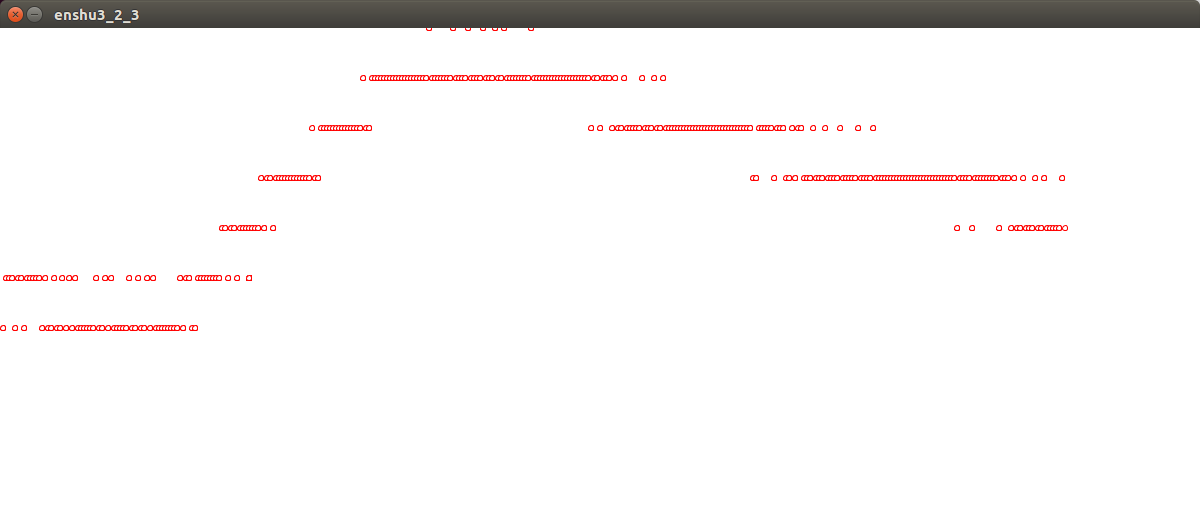
\includegraphics[width=10.0cm]{images/enshu3-2-3.png}
\caption{演習3.2.3の出力画像}
\label{fig:enshu3-2-3}
\end{center}
\end{figure}

\section{温度センサによる温度計測:複数サンプルの平均化}
課題3.2.1で作成したArduinoスケッチとProcessingスケッチを報告せよ.表示した時間-電圧グラフのスナップショットを報告せよ.サンプルの平均化を行った場合と行わなかった場合の違いについて考察せよ.

以下ソースコード\ref{code:kadai3-2-1-a},ソースコード\ref{code:kadai3-2-1-p}にそれぞれArduinoとProcessingのスケッチを示す.


\begin{lstlisting}[caption = 課題3.2.1(Arduino),label=code:kadai3-2-1-a][H]{kadai3-2-1.ino}
int sensorValue0; //センサの読み込んだ値(0~1023)
unsigned long int timePrev, timeNow;
int count; //足しこんだ回数
long int sum; //足しこんだ合計
float average; //50ms間の平均値
int intaverage;
void setup()
{
	Serial.begin(9600); // シリアル通信を 9600bps で初期化
	timePrev = millis(); // 経過時間の初期値
}
void loop()
{
  count = 0; //初期化
  sum = 0; //初期化
  while(1){
    timeNow = millis(); //現在時間を格納
    if(timeNow - timePrev <= 50){ //50ms経つまで
       int sensorValue0 = analogRead(A0); //A0の値を格納
       //double vo = sensorValue*(5.0/1024.0);
       //double Temp = (vo*1000.0 - 600.0)/10.0;
       sum += sensorValue0;
       count++;
    }
    else{
      break;
    }
  }
  average = (float)sum / (float)count;
  intaverage = (int)(average * 100);
  Serial.println(intaverage);
	Serial.write('H');
	Serial.write(timeNow >> 24); 
	// 1byte 目
	Serial.write(timeNow >>16);
	// 2byte 目
	Serial.write(timeNow >> 8);
	// 3byte 目
	Serial.write(timeNow & 255);
	// 4byte 目
	Serial.write( intaverage >> 8 );
	// 上位 1byte
	Serial.write( intaverage & 255);
	// 下位 1byte
  timePrev = timeNow; //時間の更新
}
\end{lstlisting}

\begin{lstlisting}[caption = 課題3.2.1(Processing),label=code:kadai3-2-1-p][H]
import processing.serial.*;
Serial port;
int val;
int x, y;
int high, low;
int byte1, byte2, byte3, byte4;
int time, time_min, time_max;
int period;
float f;
void setup()
{
	size(1200, 500);
	port = new Serial(this, "/dev/ttyACM0", 9600);
	period = 20000;
	// 横軸の範囲は 20,000ms 間隔
	time_min = 0;
	// 横軸の範囲の初期値
	time_max = period;// 横軸の範囲の初期値
	x = 0; y = 0;
	time = 0;
	background(255);
	frameRate(60);
}
void draw()
{
	if ( time > time_max ) { // グラフの再描画
		time_min += period; // 横軸の範囲の更新
		time_max += period; // 横軸の範囲の更新
		background(255);
	}
	x = (int)map( time, time_min, time_max, 0, width ); // x 座標値
	y = (int)map( f, 174, 184, height*0.7, 0 );
	// y 座標値
	stroke(255, 0, 0);
	ellipse(x, y, 5, 5);
}
void serialEvent(Serial p) {
	if ( p.available() >= 7 ) {
		if ( p.read() == 'H' ) {
			byte1 = p.read();
			byte2 = p.read();
			byte3 = p.read();
			byte4 = p.read();
			time = (byte1 << 24 ) + (byte2 << 16 ) + (byte3 << 8 ) + byte4; // 4 バイトデータ
			high = p.read();
			low = p.read();
			val = (high << 8 ) + low; // 2 バイトデータ
      f = (float)val /100.0; 
      println("val=",val);
      println("f=",f);
			p.clear();
		}
	}
}
\end{lstlisting}
また,以下\ref{fig:kadai3-2-1}にスナップショットを示す.

\begin{figure}[H]
\begin{center}
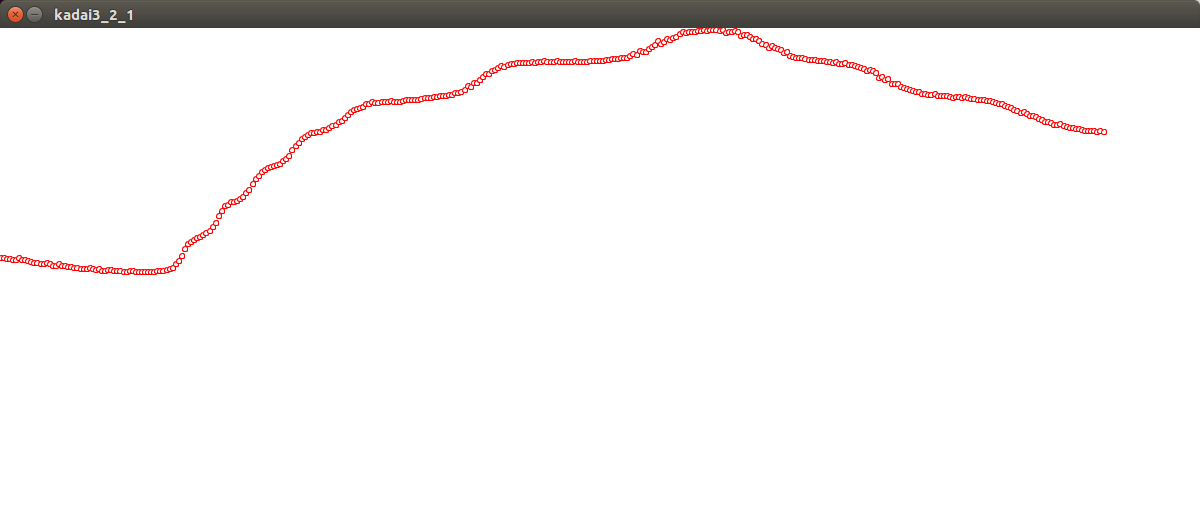
\includegraphics[width = 10.0cm]{images/kadai3-2-1.png}
\caption{課題3.2.1の出力画像}
\label{fig:kadai3-2-1}
\end{center}
\end{figure}

サンプルの平均化を行うとはずれ値を取ることがほとんどなくなる.平均化を行わない場合センサを指でつまなくても,値にある程度振れ幅があり,階段状のグラフとなるが,平均化を行うことで一定の値となる.
\section{温度センサによる温度計測:時間-温度グラフの完成}
課題3.2.2で作成したProcessingスケッチを報告せよ.表示した時間-電圧グラフのスナップショットを報告せよ.

以下ソースコード\ref{code:kadai3-2-2-p}にProcessingのスケッチを示す.

\begin{lstlisting}[caption = 課題3.2.2(Processing),label=code:kadai3-2-2-p][H]
import processing.serial.*;
Serial port;
int val; //Arduinoからの値格納用変数
int x, y; //円の中心値
int high, low; //Arduinoからの値用(上位8ビットと下位8ビット)
int byte1, byte2, byte3, byte4; //time用の4バイトの値格納用変数
int time, time_min, time_max; //現在時刻と最小値,最大値格納用変数
int t_min,t_max; //温度の最小値,最大値格納用変数
int period; //x軸の範囲設定用
float f; //valをfloat型に変換する用
int count; //y軸表示用(段階的にy軸の値を変える用)
int x_min,x_max,y_min,y_max;
void setup()
{
	size(1200, 500); //1200*500のウィンドウを生成
	port = new Serial(this, "/dev/ttyACM0", 9600);
	period = 20000; // 横軸の範囲は 20,000ms 間隔
	time_min = 0; // 横軸の範囲の初期値
	time_max = period; // 横軸の範囲の初期値
  t_min = 20; //温度の最低値
  t_max = 31; //温度の最大値
	x = 0; y = 0; //x,yの初期値
	time = 0; //timeの初期値
  count = 0; //countの初期値
  x_min = 100; //ウィンドウの一部に表示用
  x_max = 600; //ウィンドウの一部に表示用
  y_min = 100; //ウィンドウの一部に表示用
  y_max = 250; //ウィンドウの一部に表示用
	background(255); //背景を白
	frameRate(60); //フレームレート60に設定
}
void draw()
{
	if ( time > time_max ) { // グラフの再描画
		background(255); //背景を白にクリア
    /*
    count = 0; //カウントを初期化
    while ( count < (t_max - t_min +1)){ //y軸を再表示
      textSize(15); //テキストサイズを'15'に設定
      fill(0); //文字の色を黒に設定
      text("T=",30,500 - 480/(t_max - t_min)*count - 10); //"T="を表示
      text(t_min+count,50,500 - 480/(t_max - t_min)*count - 10); //20度から31度まで表示
      noFill(); //終了用
      stroke(0, 0, 255); //文字の色を青に設定
      line(0, 500 - 480/(t_max - t_min)*count-10, width,500 - 500/(t_max - t_min)*count); //y軸の線を描画
      count ++; //カウントを増やす
    }
    */
    stroke(0,0,0);
    rect(x_min,y_min,(x_max - x_min) ,(y_max - y_min));
    time_min += period; // 横軸の範囲の更新
    time_max += period; // 横軸の範囲の更新
	}
	x = (int)map( time, time_min, time_max, x_min, x_max ); // x 座標値
	y = (int)map( f, t_min, t_max, y_min, y_max ); // y 座標値
  /***************y軸の表示部分********************/
  /*
  textSize(15); //テキストサイズを'15'に設定
  fill(0); //文字の色を黒に設定
  text("T=",30,500 - 480/(t_max - t_min)*count - 10); //"T="を表示
  text(t_min+count,50,500 - 480/(t_max - t_min)*count - 10); //20度から31度まで表示
  noFill(); //終了用
  stroke(0, 0, 255); //文字の色を青に設定
  line(0, 500 - 480/(t_max - t_min)*count-10, width,500 - 500/(t_max - t_min)*count); //y軸の線を描画
  if ( count < (t_max - t_min +1)){ //31度まで表示していないなら
    count ++; //カウントを1増やす
  }
  */
  /*******************円を表示********************/
  stroke(0,0,0);
  noFill();
  rect(x_min,y_min,(x_max - x_min),(y_max - y_min));
  stroke(255, 0, 0);
	ellipse(x, y, 5, 5);
}
void serialEvent(Serial p) {
	if ( p.available() >= 7 ) {
		if ( p.read() == 'H' ) {
			byte1 = p.read(); //それぞれ1byteずつ読み込んでいく
			byte2 = p.read(); //それぞれ1byteずつ読み込んでいく
			byte3 = p.read(); //それぞれ1byteずつ読み込んでいく
			byte4 = p.read(); //それぞれ1byteずつ読み込んでいく
			time = (byte1 << 24 ) + (byte2 << 16 ) + (byte3 << 8 ) + byte4; // 4 バイトデータ
			high = p.read(); //上位8ビットを格納
			low = p.read();  //下位8ビットを格納
			val = (high << 8 ) + low; // 2 バイトデータ
      f = (float)val /100.0; //float型に直す
      println("val=",val); //値確認用
      println("f=",f); //値確認用
			p.clear();
		}
	}
}
\end{lstlisting}
また,以下\ref{fig:kadai3-2-2}にスナップショットを示す.

\begin{figure}[H]
\begin{center}
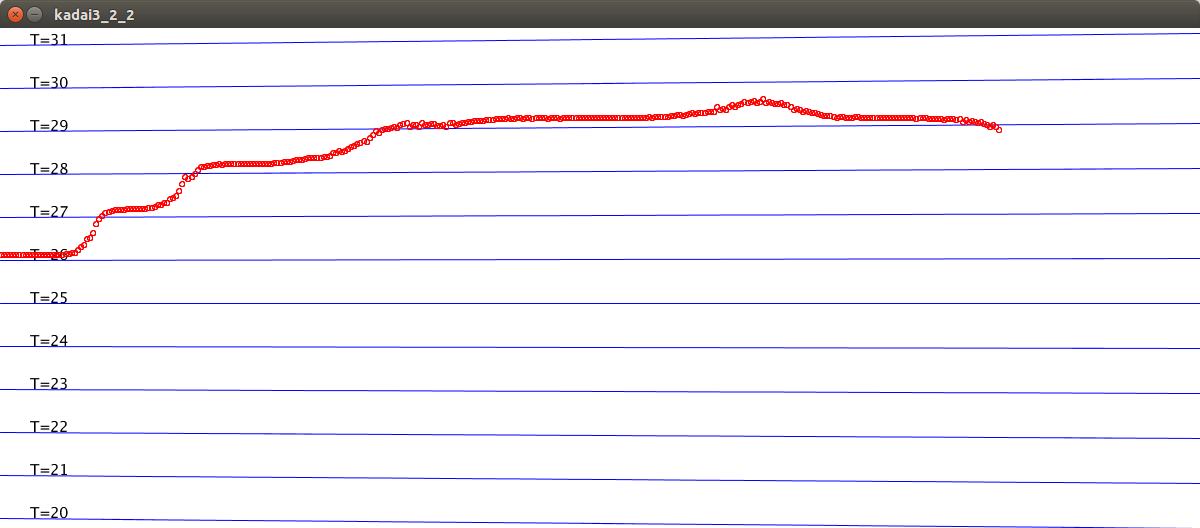
\includegraphics[width=10.0cm]{images/kadai3-2-2.png}
\caption{課題3.2.2の出力画像}
\label{fig:kadai3-2-2}
\end{center}
\end{figure}

\section{温度センサによる温度計測:グラフ配置}
課題3.2.3で作成したProcessingスケッチを報告せよ.表示した時間-電圧グラフのスナップショットを報告せよ.

以下ソースコード\ref{code:kadai3-2-3-p}にProcessingのスケッチを示す.

\begin{lstlisting}[caption = 課題3.2.3(Processing),label=code:kadai3-2-3-p][H]
import processing.serial.*;
Serial port;
int val; //Arduinoからの値格納用変数
int x, y; //円の中心値
int high, low; //Arduinoからの値用(上位8ビットと下位8ビット)
int byte1, byte2, byte3, byte4; //time用の4バイトの値格納用変数
int time, time_min, time_max; //現在時刻と最小値,最大値格納用変数
int t_min,t_max; //温度の最小値,最大値格納用変数
int period; //x軸の範囲設定用
float f; //valをfloat型に変換する用
int count; //y軸表示用(段階的にy軸の値を変える用)
int x_min,x_max,y_min,y_max;
void setup()
{
	size(1200, 500); //1200*500のウィンドウを生成
	port = new Serial(this, "/dev/ttyACM0", 9600);
	period = 20000; // 横軸の範囲は 20,000ms 間隔
	time_min = 0; // 横軸の範囲の初期値
	time_max = period; // 横軸の範囲の初期値
  t_min = 20; //温度の最低値
  t_max = 31; //温度の最大値
	x = 0; y = 0; //x,yの初期値
	time = 0; //timeの初期値
  count = 0; //countの初期値
  x_min = 100; //ウィンドウの一部に表示用
  x_max = 600; //ウィンドウの一部に表示用
  y_min = 100; //ウィンドウの一部に表示用
  y_max = 250; //ウィンドウの一部に表示用
	background(255); //背景を白
	frameRate(60); //フレームレート60に設定
}
void draw()
{
	if ( time > time_max ) { // グラフの再描画
		background(255); //背景を白にクリア
    
    count = 0;
    while ( count < (t_max - t_min + 1)){
      textSize(13); //テキストサイズを'15'に設定
      fill(0); //文字の色を黒に設定
      text("T=",110,150 - 150/(t_max - t_min)*count + 100); //"T="を表示
      text(t_min+count,130,150 - 150/(t_max - t_min)*count +100); //20度から31度まで表示
      noFill(); //終了用
      stroke(0, 0, 255); //文字の色を青に設定
      line(x_min, 150 - 150/(t_max - t_min)*count + 100, x_max,150 - 150/(t_max - t_min)*count+ 100); //y軸の線を描画
      count++;
    }
    stroke(0,0,0);
    rect(x_min,y_min,(x_max - x_min) ,(y_max - y_min));
    time_min += period; // 横軸の範囲の更新
    time_max += period; // 横軸の範囲の更新
	}
	x = (int)map( time, time_min, time_max, x_min, x_max ); // x 座標値
	y = (int)map( f, t_min, t_max, y_max, y_min ); // y 座標値
  /***************y軸の表示部分********************/
  
  textSize(13); //テキストサイズを'15'に設定
  fill(0); //文字の色を黒に設定
  text("T=",110,150 - (150/(t_max - t_min)*count )+ 100); //"T="を表示
  text(t_min+count,130,150 - 150/(t_max - t_min)*count +100); //20度から31度まで表示
  noFill(); //終了用
  stroke(0, 0, 255); //文字の色を青に設定
  line(x_min, 150 - 150/(t_max - t_min)*count + 100, x_max,150 - 150/(t_max - t_min)*count+ 100); //y軸の線を描画
  if ( count < (t_max - t_min)){ //31度まで表示していないなら
    count ++; //カウントを1増やす
  }
  
  /*******************円を表示********************/
  stroke(0,0,0);
  noFill();
  rect(x_min,y_min,(x_max - x_min),(y_max - y_min));
  stroke(255, 0, 0);
	ellipse(x, y, 5, 5);
}
void serialEvent(Serial p) {
	if ( p.available() >= 7 ) {
		if ( p.read() == 'H' ) {
			byte1 = p.read(); //それぞれ1byteずつ読み込んでいく
			byte2 = p.read(); //それぞれ1byteずつ読み込んでいく
			byte3 = p.read(); //それぞれ1byteずつ読み込んでいく
			byte4 = p.read(); //それぞれ1byteずつ読み込んでいく
			time = (byte1 << 24 ) + (byte2 << 16 ) + (byte3 << 8 ) + byte4; // 4 バイトデータ
			high = p.read(); //上位8ビットを格納
			low = p.read();  //下位8ビットを格納
			val = (high << 8 ) + low; // 2 バイトデータ
      f = (float)val /100.0; //float型に直す
      println("val=",val); //値確認用
      println("f=",f); //値確認用
			p.clear();
		}
	}
}
\end{lstlisting}
また,以下\ref{fig:kadai3-2-3}にスナップショットを示す.

\begin{figure}[H]
\begin{center}
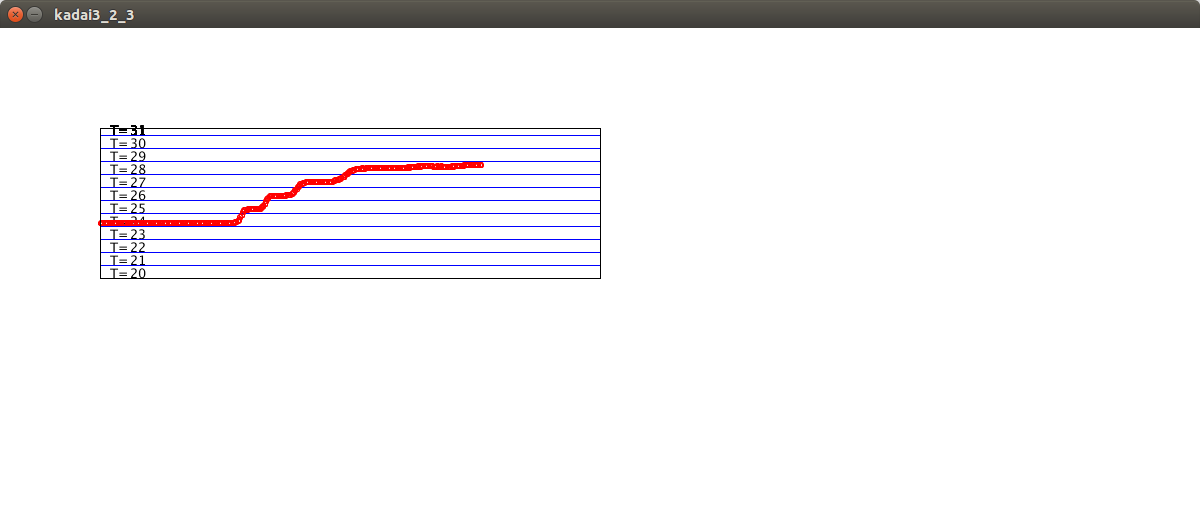
\includegraphics[width=10.0cm]{images/kadai3-2-3.png}
\caption{課題3.2.3の出力画像}
\label{fig:kadai3-2-3}
\end{center}
\end{figure}

\end{document}
